\chapter{BER理論値を指標とする送信電力制御適用型使用チャネル足切りアルゴリズム
}
本章では,第3章で提案した既存のPPLアルゴリズムについて,研究背景,問題提起をしたのち,これに対する
改善案として3つの内容を検証する.1つ目に伝搬路のSN比が既知であるとしたときのBER理論値を基準とした
獲得固有ベクトル足切りアルゴリズム,2つ目に送信電力分配による理論BER最小化,そして3つ目に,
以上の2つの内容を同時適用した場合を検証する.

\section{研究背景}
第3章では,チャネル推定を行った後に合成チャネル行列を計算して固有値分解する
従来のVCに対して,べき乗法を基本原理とするPPLによる固有ベクトル獲得を提案した.
PPLの最大の特徴は,チャネル推定・合成チャネル行列計算・固有値分解の膨大な演算を,極めて簡単な
非線形処理と無線機間反復処理に置き換えることにある.つまり,伝搬路情報を経由せずに
直接的に固有値・固有ベクトルを求めることができる点に強みがある.
しかし,現在のPPLにおける固有値・固有ベクトルの獲得にかかる無線機間往復数では,実用には十分でないという
問題点がある.固有値問題の性質上,解法には反復解法を用いざるを得ない.PPLではべき乗法を
基本原理としているため,ある程度の反復回数の増加は避けられない.また,VCという方式自体としても
いくつかの課題を有している.その一つに,固有ベクトルに対応する固有値の大きさが,
そのままそのチャネルの利得になっているという特徴上,利得の小さい
チャネルを使用して伝送したデータが,他のチャネルを使用した場合と比較して誤りやすくなるという
問題がある.本章では,上記の二つの問題点に焦点を当て,3つの内容に分けて検証を行う.

\section{検討内容}
ここでは,全部で3つの内容について検討を行う.まず,1つ目としてPPLの課題である無線機間往復数に
対して,一定の通信品質を満たさないチャネルをBER理論値に基づいて足切りすることによる往復数削減
を検証する.2つ目に,VCの課題として挙げた低利得チャネルの誤り率増加減少に対して,送信電力制御
適用によるBER理論値最小化を行う.最後に,1つ目の足切りアルゴリズムに対して,送信電力制御を
組み込んだ場合について検証を行っていく.

\subsection{BER理論値を指標とする使用チャネル足切りアルゴリズム}
ここでは,BER理論値を指標とする使用チャネル足切りアルゴリズムについて解説を行う.
従来のPPLでは,反復処理を行う際,求めたい固有ベクトルの数をあらかじめ
決めたうえで,すべての固有ベクトルが収束するまで反復を行っている.しかし,これは反復回数の面
では無駄が多い.理由として主に以下の3つが挙げられる.1つ目に,べき乗法の特徴として,固有値を大きい順に並べた際に,隣の
固有値との比が大きいほど固有ベクトルの収束が速くなり,逆に小さいほど遅くなるという点が挙げられる.
つまり,求めたい固有ベクトルのうち小さい固有値に対応するものほど,必然的に前の固有値との
比が小さくなるため,獲得までに多くの反復回数を
要することになる.2つ目に,3.5節で説明したように,第2固有ベクトルの獲得では第1固有ベクトルを,
第3固有ベクトルの獲得では第1・第2固有ベクトルを必要とするように,
各固有ベクトルの獲得精度はそれ以前の固有ベクトルの獲得精度の影響を強く受ける.そのため,
後半になるにしたがって,固有ベクトルの獲得精度が低くなり,全体として見たとき拡散符号全体の
直交性が悪化してしまう.3つ目に,固有値が小さい,後半のベクトルほど誤り率が高くなるという
点が挙げられる.VCにおいて,固有値の大きさは各チャネルの利得に対応している.そのため,
固有値の小さいチャネルほど,受信される信号電力が低くなるので,SN比が低下し誤りやすくなるという
特徴がある.上記の理由から,小さい固有値に対応する後半の固有ベクトルを,適切に足切りする
ことができれば,実質的な通信品質を損なわずに不要な反復回数を削減できると考えられる.

図 \ref{figCutoff}に足切りアルゴリズムの概略図,図 \ref{figCutoffFlow}に足切りアルゴリズムのフローチャートを示す.
なお,図 \ref{figCutoff}の固有ベクトル導出に必要な処理は簡略版を示している.
\begin{figure}
    \centering
    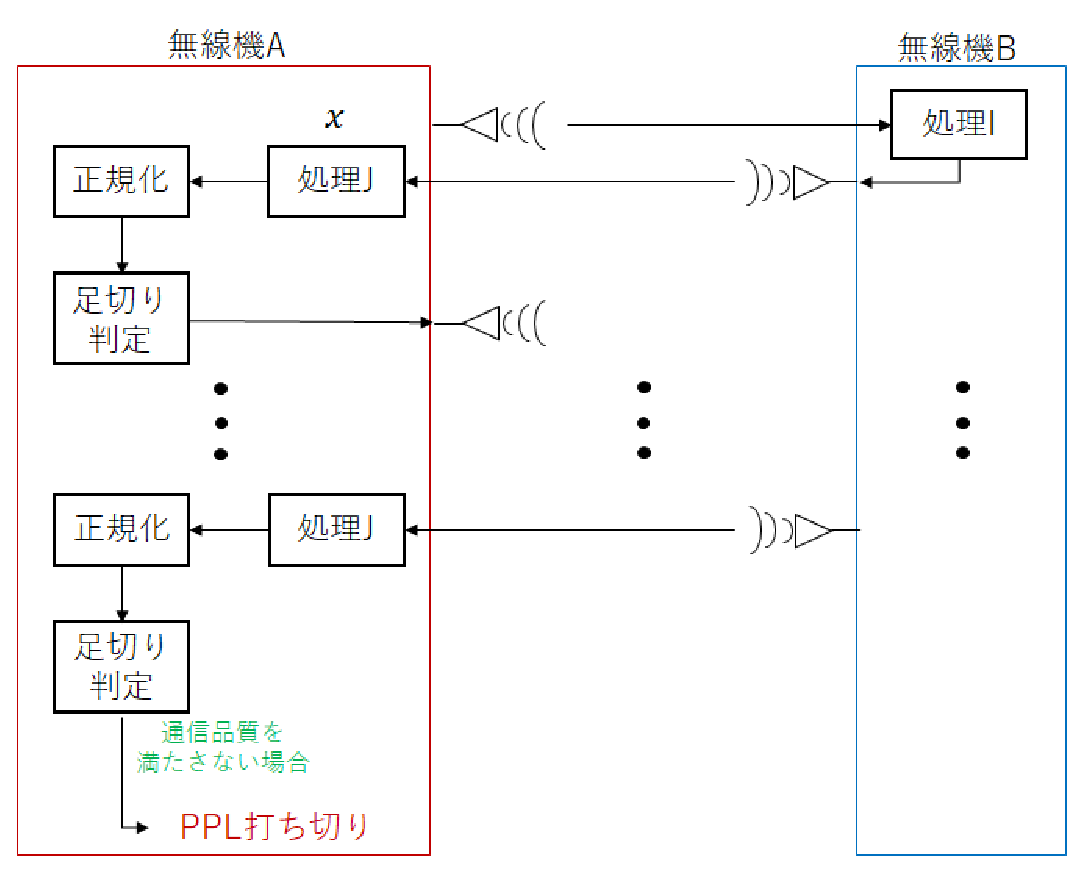
\includegraphics[width=\linewidth]{chapter4/figure/Cutoff.eps}
    \caption{足切りアルゴリズム概略図}
    \label{figCutoff}
\end{figure}
\begin{figure}
    \centering
    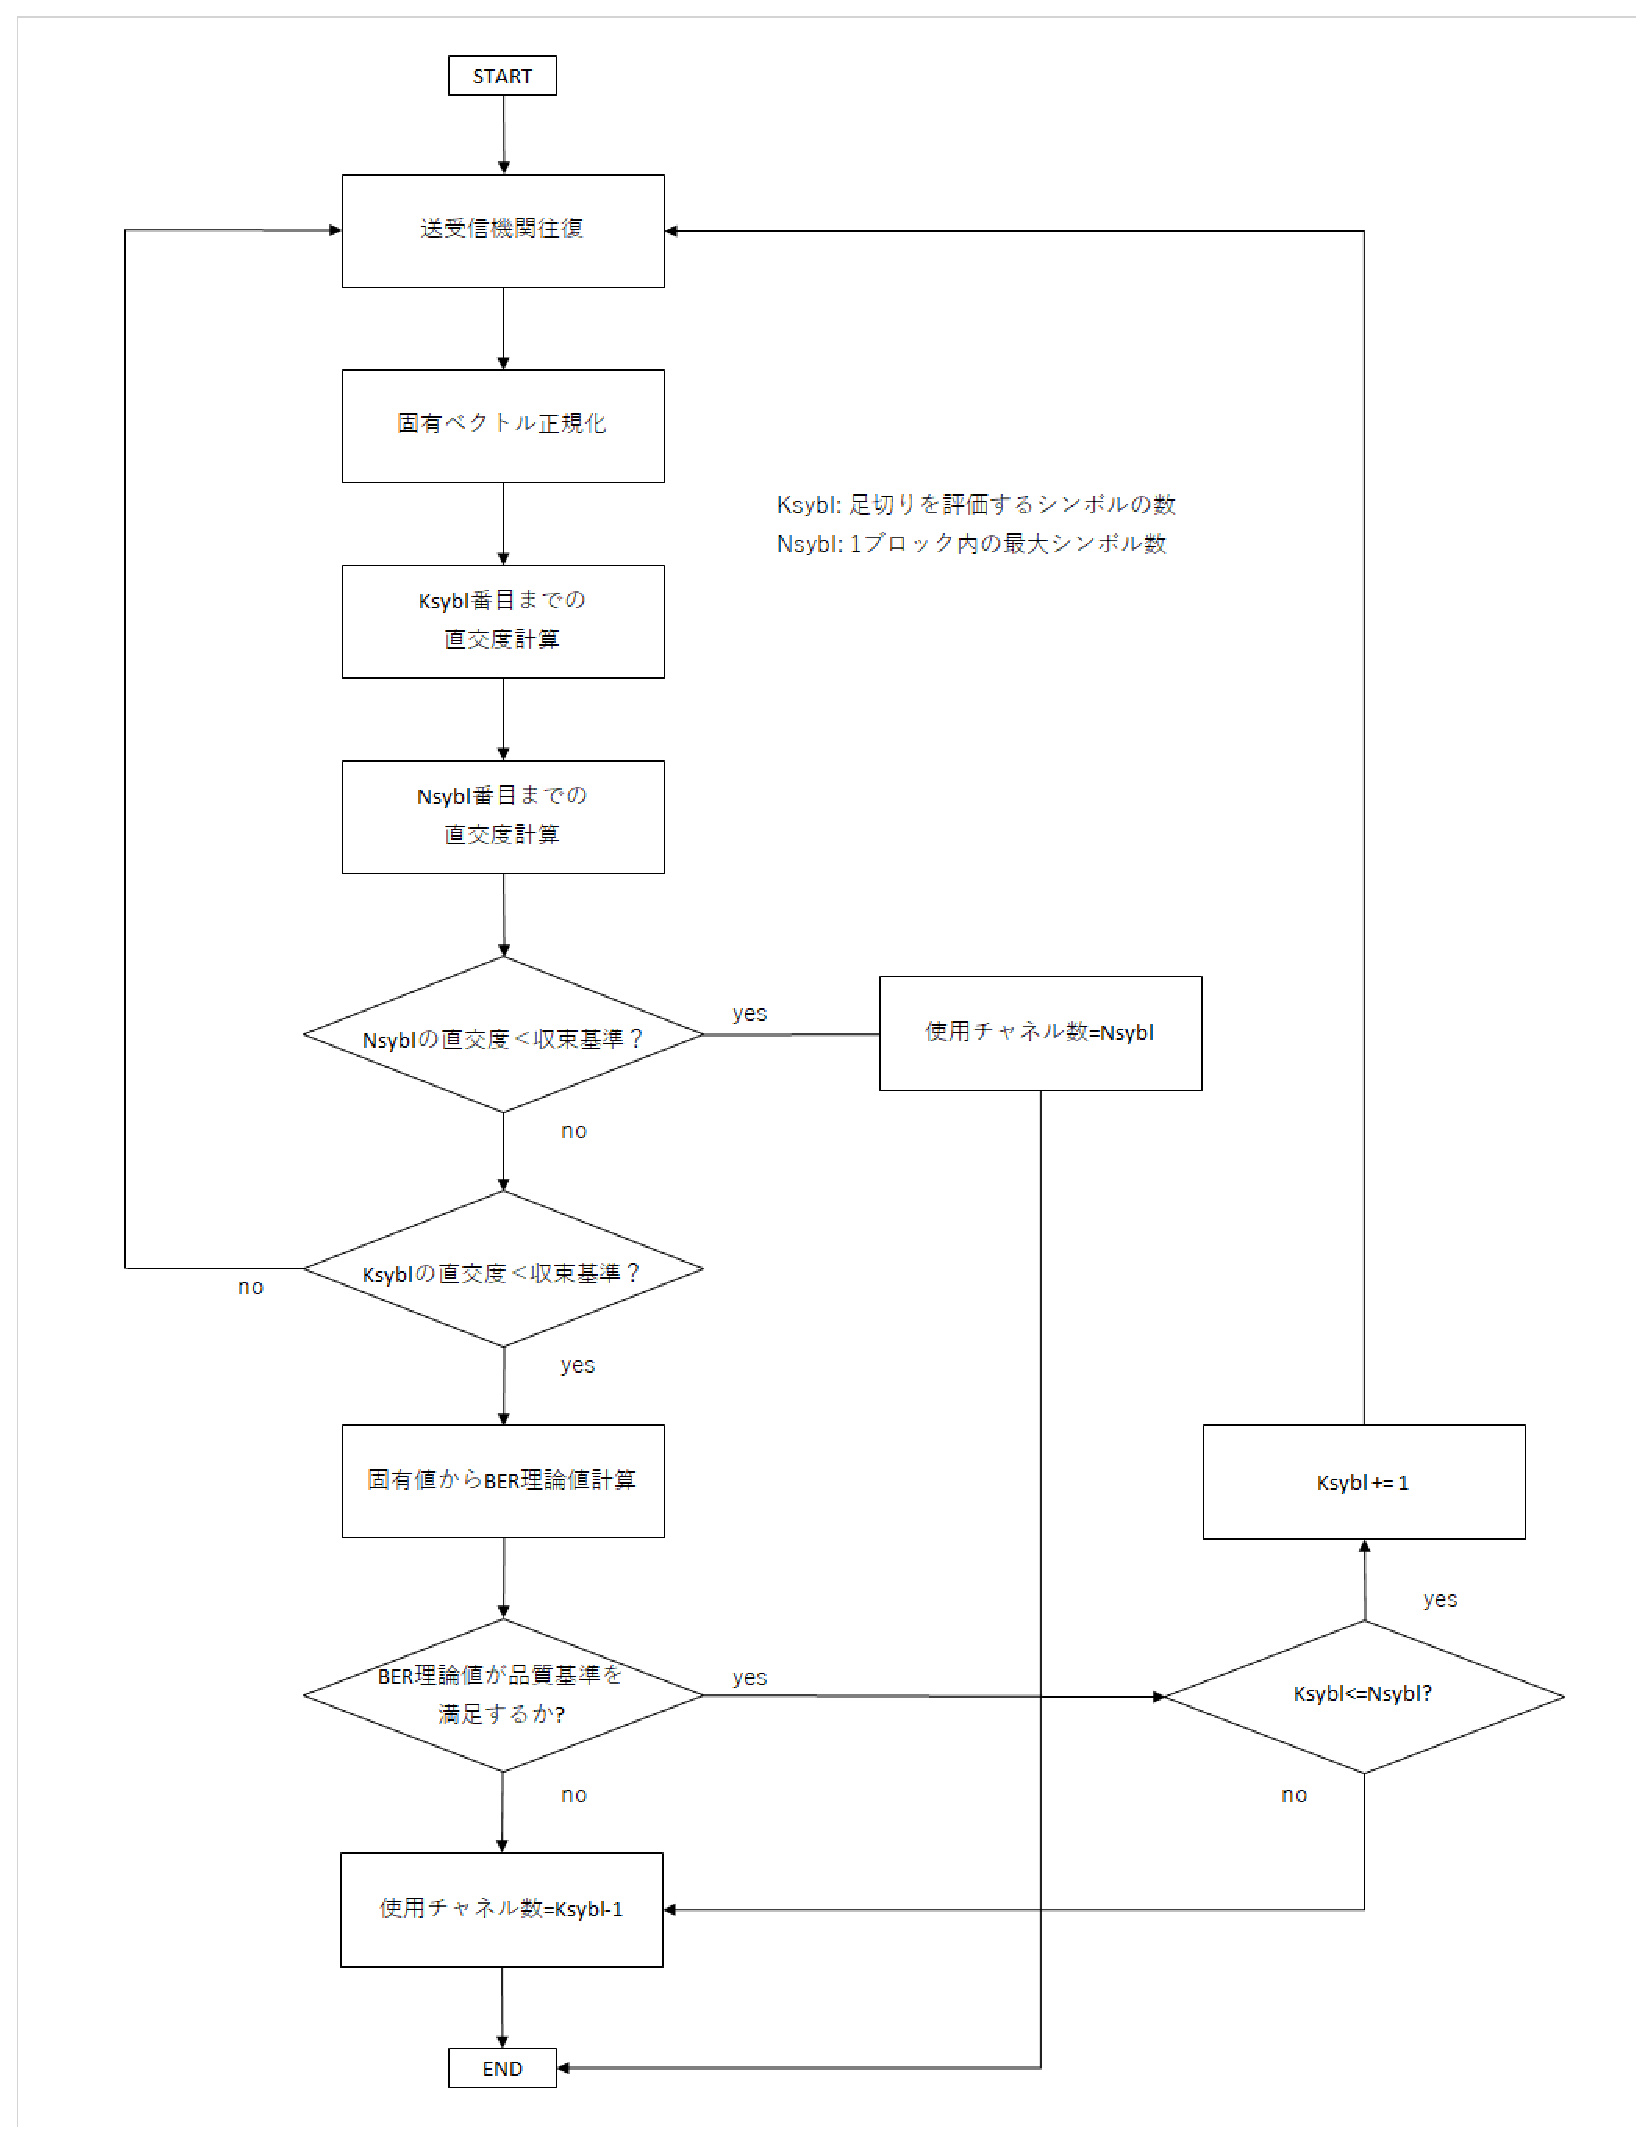
\includegraphics[width=0.95\linewidth]{chapter4/figure/CutoffFlow.eps}
    \caption{足切りアルゴリズムフローチャート}
    \label{figCutoffFlow}
\end{figure}
図 \ref{figCutoffFlow}のKsyblは足切り評価を行う固有ベクトル数に
なっている.また,固有ベクトルの収束判定基準に使用する直交度は以下のように定義するものとする.\\
\vspace{5mm}
(例) \quad 固有ベクトルが$\bm{u_1,u_2,u_3}$の3つの場合を考える.
\begin{equation}
    直交度 = \left|\bm{u_1^Hu_2}\right|+\left|\bm{u_1^Hu_3}\right|+\left|\bm{u_2^Hu_3}\right|
\end{equation}

具体的にどのように足切り判定が行われるか図 \ref{figCutoffFlow}をもとに説明する.
当該アルゴリズムは大きく分けて3つの段階に分かれている.
一つ目に無線機間往復,2つ目に獲得固有ベクトルの収束判定,そして3つ目に,収束した固有ベクトルを
用いた場合の通信品質がある基準を満たしているかのBER判定である.
まず,1つ目の無線機間往復について,これは第3章に説明したように非線形処理と正規化を伴う一連の
処理である.次に収束判定についてだが,これはKsybl番目までの固有ベクトルの直交度を求めて,
求めた値が事前に設定した収束基準を満たせば収束したとするものである.収束基準は実験的に求めた
値を使用する.
\begin{equation}
    Ksybl番目までの直交度 \leq 収束基準
\end{equation}
となれば,Ksybl番目までの固有ベクトルが求まったと判断する.
最後に,2つ目の収束判定を合格した固有ベクトルを使用した場合のBER理論値を計算し,
として無線機間往復を打ち切る.ここで,Ksybl番目までの固有ベクトルを使用する際の
BER理論値は以下の式,
\begin{equation}
    BER = \frac{1}{Ksybl}\sum_{i=1}^{Ksybl} \frac{1}{2}erfc\left( \sqrt{\lambda_i\frac{E_b}{N_0}} \right)
\end{equation}
で与えられる.上記のBER理論値はQPSKを変調方式として用いた場合のものである.
 \cite{akaiwa}なお,$erfc(x)$は相補誤差関数,$E_bN_0$は伝搬路の1ビット当たりの信号電力
対雑音電力比で,$E_bN_0$は既知とする.このBER理論値が,
\begin{equation}
    BER > BER基準
\end{equation}
を満たす場合,Ksybl番目を含めた通信品質が所望品質を満たさないとして,Ksybl-1番目までを
使用チャネルとしてPPLを打ち切る.ここで,BER基準は$10^{-2}$以下の誤り率であれば,
誤り訂正符号適用時に誤りを復元できるとして,$BER基準=10^{-2}$に設定する.
以上が当該アルゴリズムの解説になる.

\subsection{送信電力制御を用いたBER理論値最小化}
ここでは,送信電力制御によるBER理論値最小化手法について解説を行う.
BER理論値の最小化は,各チャネルに割り当てられる送信電力を変数としたとき,目的関数である
BER理論値を最小とするような送信電力の組み合わせを見つける最適化問題を解くことで得られる.
以下で,式を用いて具体的に説明していく.

まず,変調方式にQPSKを使用する際のBER理論値は(4.3)式と同様に以下で表される.
\begin{equation}
    \frac{1}{N} \sum_{i=1}^N \frac{1}{2}erfc\left( \sqrt{\lambda_i\frac{E_b}{N_0}} \right)
\end{equation}
\begin{equation}
    \left[
        \begin{array}{l}
            N:1ブロック当たりのシンボル数 \\
            \lambda_i:i番目の固有ベクトルに対応する固有値 \\
            E_bN_0:平均E_bN_0
        \end{array}
    \right. \nonumber
\end{equation}
ここに,送信電力$p$を挿入することで,最小化する目的関数,
\begin{equation}
    f(p_1,p_2,\ldots,p_N) = \frac{1}{N} \sum_{i=1}^N \frac{1}{2}erfc\left( \sqrt{p_i\lambda_i\frac{E_b}{N_0}} \right)
\end{equation}
を得る.
また,送信電力$p_i$に関して,全送信電力の合計がNになるということと,各送信電力が非負であるので,
\begin{eqnarray}
    h(p_1,p_2,\ldots,p_N) = \sum_{i=1}^N p_i-N=0 \\
    p_i \geq 0 \hspace{10mm} (i=1,2,\ldots,N)
\end{eqnarray}
の等式制約,不等式制約を考慮する必要がある.(4.7),(4.8)式の制約条件から,この最適化問題はKKT条件と
なっている.以上の最適化問題をラグランジュの未定乗数法を用いて解いていく.
ラグランジュの未定乗数法は2.4.2節で示した通りだが,ここでは問題を簡単にするために一旦
(4.8)式は無視し,等式制約のみの場合で考える.これによって,一般的に解くことが難しいとされる
KKT条件を等式条件のみの最適化問題に帰着させる.さらに,目的関数fが相補誤差関数で表され積分を
含むため,計算が非常に困難になる.そこで,この関数fをチェルノフ限界(Chernoff bound) \cite{akaiwa},
\begin{equation}
    Q(x) = \frac{1}{2}erfc\left( \frac{x}{\sqrt{2}} \right) \leq \exp\left( -\frac{x^2}{2} \right)
\end{equation}
を用いて以下のように近似する.
\begin{equation}
    \frac{1}{N}\sum_{i=1}^N \frac{1}{2}erfc\left( \sqrt{p_i\lambda_i\frac{E_b}{N_0}} \right)
    \leq \frac{1}{N}\sum_{i=1}^N exp \left( -p_i\lambda_i\frac{E_b}{N_0} \right)
\end{equation}
ラグランジュ関数$L$は(2.11)式より,
\begin{equation}
    L(p_1,p_2,\ldots,p_N,\mu) = f(p_1,p_2,\ldots,p_N)-\mu h(p_1,p_2,\ldots,p_N)
\end{equation}
で表され,
\begin{equation}
    \frac{\partial L}{\partial p_i}=\frac{\partial L}{\partial \mu}=0 \hspace{10mm} 
    (i=1,2,\ldots,N)
\end{equation}
を解くことで解が得られる.(4.12)式より,これを(4.6)式,(4.7)式に当てはめると,
\begin{eqnarray}
    \frac{\partial L}{\partial p_i}&=&-\frac{\lambda_i}{N}\frac{E_b}{N_0}
    exp\left( -\lambda_i\frac{E_b}{N_0}p_i \right)-\mu=0 \hspace{10mm} (i=1,2,\ldots,N) \\
    \frac{\partial L}{\partial \mu}&=&p_1+p_2+\cdots+p_N-N=0
\end{eqnarray}
となる.(4.13)式より,
\begin{eqnarray}
    -\frac{\lambda_i}{N}\frac{E_b}{N_0}
    exp\left( -\lambda_i\frac{E_b}{N_0}p_i \right)-\mu &=& 0 \nonumber \\
    exp\left( -\lambda_i\frac{E_b}{N_0}p_i \right) &=& -\frac{N}{\lambda_i\frac{E_b}{N_0}}\mu \nonumber \\
    -\lambda_i\frac{E_b}{N_0}p_i &=& ln\left( -\frac{N}{\lambda_i\frac{E_b}{N_0}}\mu \right) \hspace{10mm} (両辺lnをとる) \nonumber \\
    -\lambda_i\frac{E_b}{N_0}p_i &=& ln\left( -\mu \right) + ln\left( \frac{N}{\lambda_i\frac{E_b}{N_0}} \right) \nonumber \\
    p_i &=& -\frac{1}{\lambda_i\frac{E_b}{N_0}}\left( ln\left( -\mu \right) + 
    ln\left( \frac{N}{\lambda_i\frac{E_b}{N_0}} \right) \right) \hspace{10mm} (i=1,2,\ldots,N)
\end{eqnarray}
となる.(4.15)式を(4.14)式に代入すると,
\begin{eqnarray}
    -\frac{1}{\frac{E_b}{N_0}}\sum_{i=1}^N \frac{1}{\lambda_i}
    \left( ln\left( -\mu \right)+ln\left( \frac{N}{\lambda_i\frac{E_b}{N_0}} \right) \right)-N &=& 0 \nonumber \\
    -\frac{ln(-\mu)}{\frac{E_b}{N_0}}\sum_{i=1}^N \frac{1}{\lambda_i} &=& 
    N+\frac{1}{\frac{E_b}{N_0}}\sum_{i=1}^N \frac{1}{\lambda_i}ln\left( \frac{N}{\lambda_i\frac{E_b}{N_0}} \right) \nonumber \\
    ln(-\mu) &=& -\frac{E_b}{N_0}\frac{1}{\sum_{i=1}^N \frac{1}{\lambda_i}} 
    \left( N+\frac{1}{\frac{E_b}{N_0}}\sum_{i=1}^N \frac{1}{\lambda_i}ln\left( \frac{N}{\lambda_i\frac{E_b}{N_0}} \right) \right)
\end{eqnarray}
と,$ln(-\mu)$が求められる.また,以上より(4.15)式に(4.16)式を代入することで各$p_i$を求めることができる.

ここまでは,(4.8)式の不等式制約を無視して計算を行ったが,実際に(4.15)式を解くと,
\begin{equation}
    p_k < 0 \hspace{10mm} (1 \leq k \leq N)
\end{equation}
のような$p_k$が存在する場合がある.送信電力が負になることはありえないので,
$p_k$のうち最小の$p_k$を$p_{min}$とおいて,
\begin{equation}
    p_i = p_i-(p_{min}-c) \hspace{10mm} (i=1,2,\ldots,N)
\end{equation}
のように全体を正方向に$p_{min}-c$だけシフトさせる.この時$c$は任意の最小送信電力とする.
全体をシフトさせた後,送信電力の合計がNになるように全体を正規化してやれば,各$p_i$の相対的な
大小関係を保ったまま,負となる変数を無くすことができる.つまり,(4.8)式の不等式制約も満足
させることができる.以上が,BER理論値を最小化する送信電力制御の方針である.

\subsection{送信電力制御適用時の使用チャネル足切りアルゴリズム}
ここでは,4.2.1節,4.2.2節で説明した足切りアルゴリズムと送信電力最適化の2つを同時適用した場合に,
送信電力制御によって所望の通信品質を満足するチャネル数を最大化しつつ,不要なチャネルを足切りする
アルゴリズムを提案する.
図 \ref{figCombFlow}にフローチャートを示す.
\begin{figure}
    \centering
    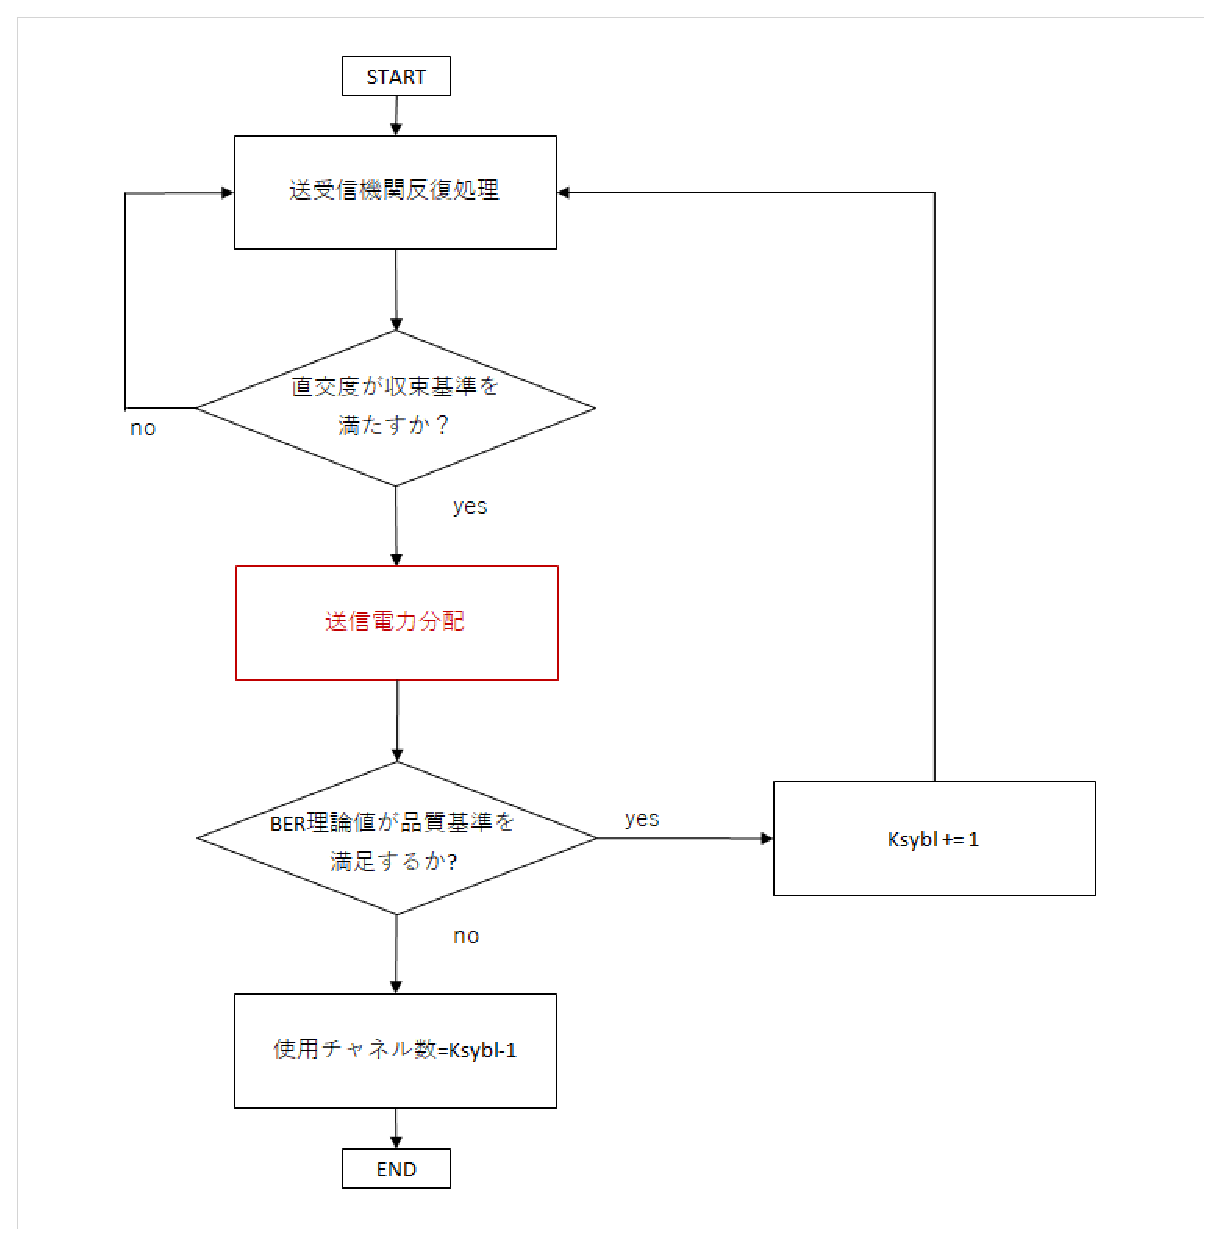
\includegraphics[width=0.95\linewidth]{chapter4/figure/CombFlow.eps}
    \caption{送信電力制御適用時の足切りアルゴリズムフローチャート}
    \label{figCombFlow}
\end{figure}
基本的には4.2.1節で解説した足切りアルゴリズムと同じだが,図中の赤い四角で囲われた送信電力分配
が追加されている.4.2.1節のアルゴリズムでは,獲得したKsybl個の固有ベクトルを使用して
通信した際のBER理論値を求め,この理論値があらかじめ設定した通信品質基準を満足するか判断した.
ここで送信電力分配を適用することによって,獲得したKsybl個の固有ベクトルを用いたBER理論値を
最小化することができる.BER理論値が最小化されるということは,送信電力分配の次の項目である
通信品質基準が満足されやすくなるということである.つまり,使用可能チャネル数が最大化されるので,
実質的に通信速度を最大にしつつ,足切りによって反復回数を削減することができる.

\section{検証}
ここでは,4.2.1節,4.2.2節,4.2.3節で解説した3つの内容についてシミュレーションを用いた検討を
行う.

\subsection{BER理論値を指標とする使用チャネル足切りアルゴリズム}
ここでは,4.2.1節で解説したBER理論値を指標とした固有ベクトル(使用チャネル)足切りアルゴリズム
について検証を行う.足切りを行わない場合と比較して,実質的に使用できるチャネル数を減らさずに
無線機間反復回数のみ削減できることを示す.

\subsubsection{シミュレーション諸元}
まず,図 \ref{figCutoffFlow}にあるように,固有ベクトルの収束判断に使用する収束基準と,
BER理論値を評価する際の通信品質基準の2つを決定する必要がある.通信品質基準については,
$10^{-2}$以下のBERであれば,誤り訂正符号を付加すれば誤り率を0にすることができると仮定して,
\begin{equation}
    品質基準=10^{-2}
\end{equation}
とするものとする.

収束基準については,直交度について検証を行うことによって実験的に求めていく.
まず,横軸を直交度,縦軸をBERとした時に直交度とBERがどのような関係にあるかをシミュレーションを用いて
検証する.表 \ref{tabCutoff1}にシミュレーション諸元を示す.
諸元に示した通り,PPLのシミュレーションについては本章全体を通して,雑音が無い,もしくはほとんど無い環境で行われるものとする.

\begin{table}[ht]
    \begin{tabular}{|c|c|} \hline
        1ブロック当たりのシンボル数 & 32 \\ \hline
        マルチパス数 & 4 \\ \hline
        変調方式 & QPSK \\ \hline
        チャネルモデル & 準静的レイリーフェージング \\ \hline
        PPL時の雑音考慮 & 無し \\ \hline
        $E_bN_0$ & 0,10,20,30[dB] \\ \hline
    \end{tabular}
    \centering
    \caption{直交度とBERの関係 シミュレーション諸元}
    \label{tabCutoff1}
\end{table}

シミュレーション結果を図 \ref{figCutoffSim1}に示す.

\begin{figure}[ht]
    \centering
    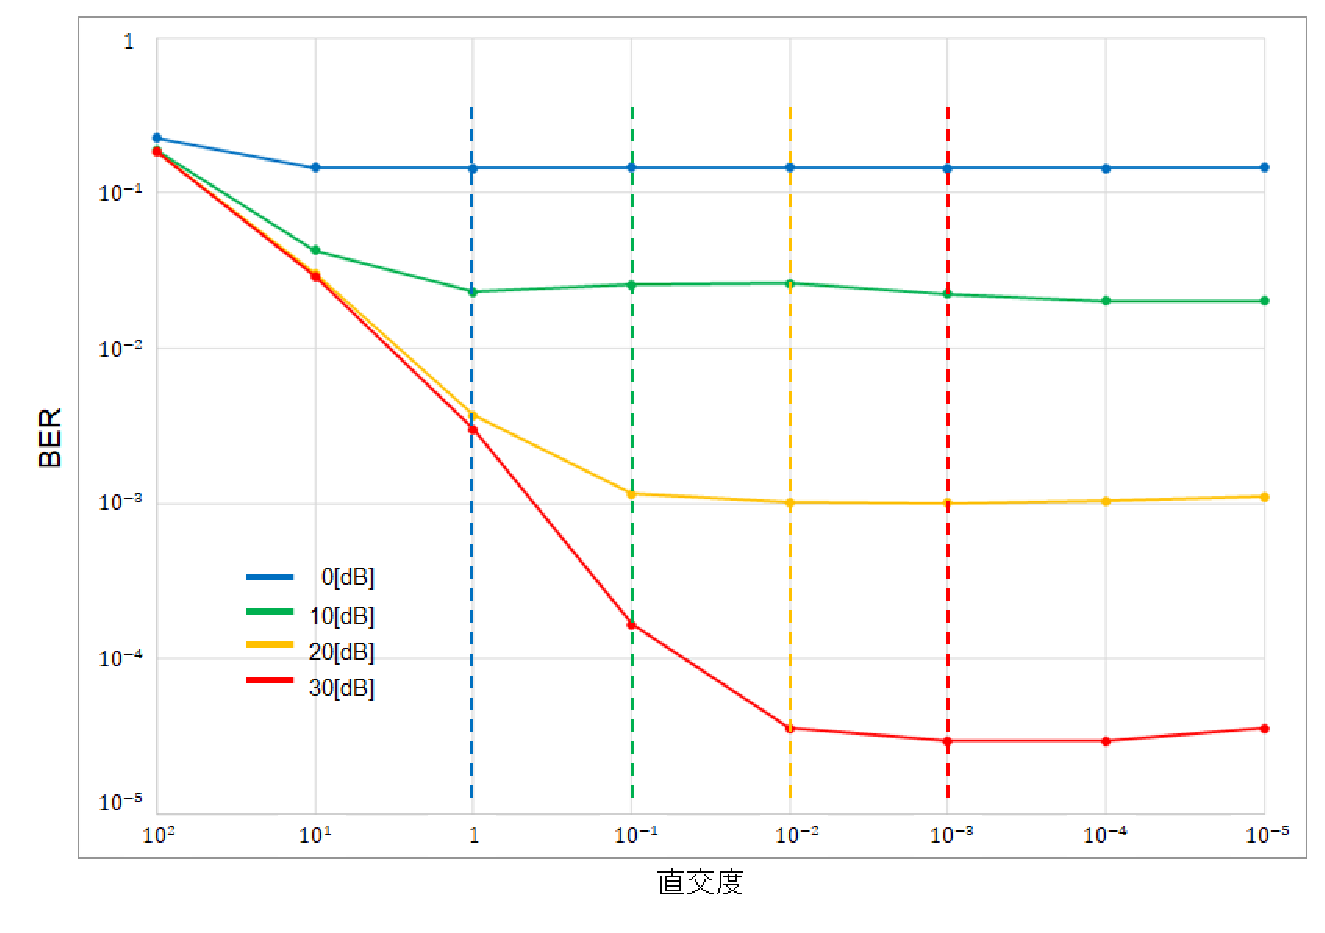
\includegraphics[width=0.95\linewidth]{chapter4/figure/CutoffSim1.eps}
    \caption{直交度とBERの関係}
    \label{figCutoffSim1}
\end{figure}

図 \ref{figCutoffSim1}を見てみると,それぞれの$E_bN_0$の条件において,
ある値からBERが改善しなくなっている.このラインを各$E_bN_0$について色付きの点線で
示している.このBERが打ち止めとなる点と$E_bN_0$の関係を表 \ref{tabCutoff2}にまとめた.

\begin{table}[ht]
    \begin{tabular}{|c|c|} \hline
        $E_bN_0$ & 打ち止め点 \\ \hline
        0 & 1 \\ \hline
        10 & 0.1 \\ \hline
        20 & 0.01 \\ \hline
        30 & 0.001 \\ \hline
    \end{tabular}
    \centering
    \caption{$E_bN_0$とBER打ち止め点の関係}
    \label{tabCutoff2}
\end{table}

表 \ref{tabCutoff2}より,各$E_bN_0$と直交度が打ち止めとなる点の関係は,
\begin{equation}
    E_bN_0の打ち止め点 = 10*exp(-0.23E_bN_0)
\end{equation}
のように数式で表すことができる.これより,各$E_bN_0$の条件についての収束基準を,
\begin{equation}
    収束基準 = exp(-0.23E_bN_0)
\end{equation}
というように設けることとする.なお,(4.21)式の収束基準は,ある程度の余裕を持たせるために
(4.20)式の結果を0.1倍したものを使用している.
図 \ref{figCutoffSim1}の結果はマルチパス数が4の場合だったが,マルチパス数が変化した場合についても
直交度とBERの関係がどうなるのか検証する必要がある.
検証結果を図 \ref{figCutoffSim2}に示す.なお,諸元については$E_bN_0=10[dB]$とする以外は
表 \ref{tabCutoff1}と同じ条件とする.

\begin{figure}[ht]
    \centering
    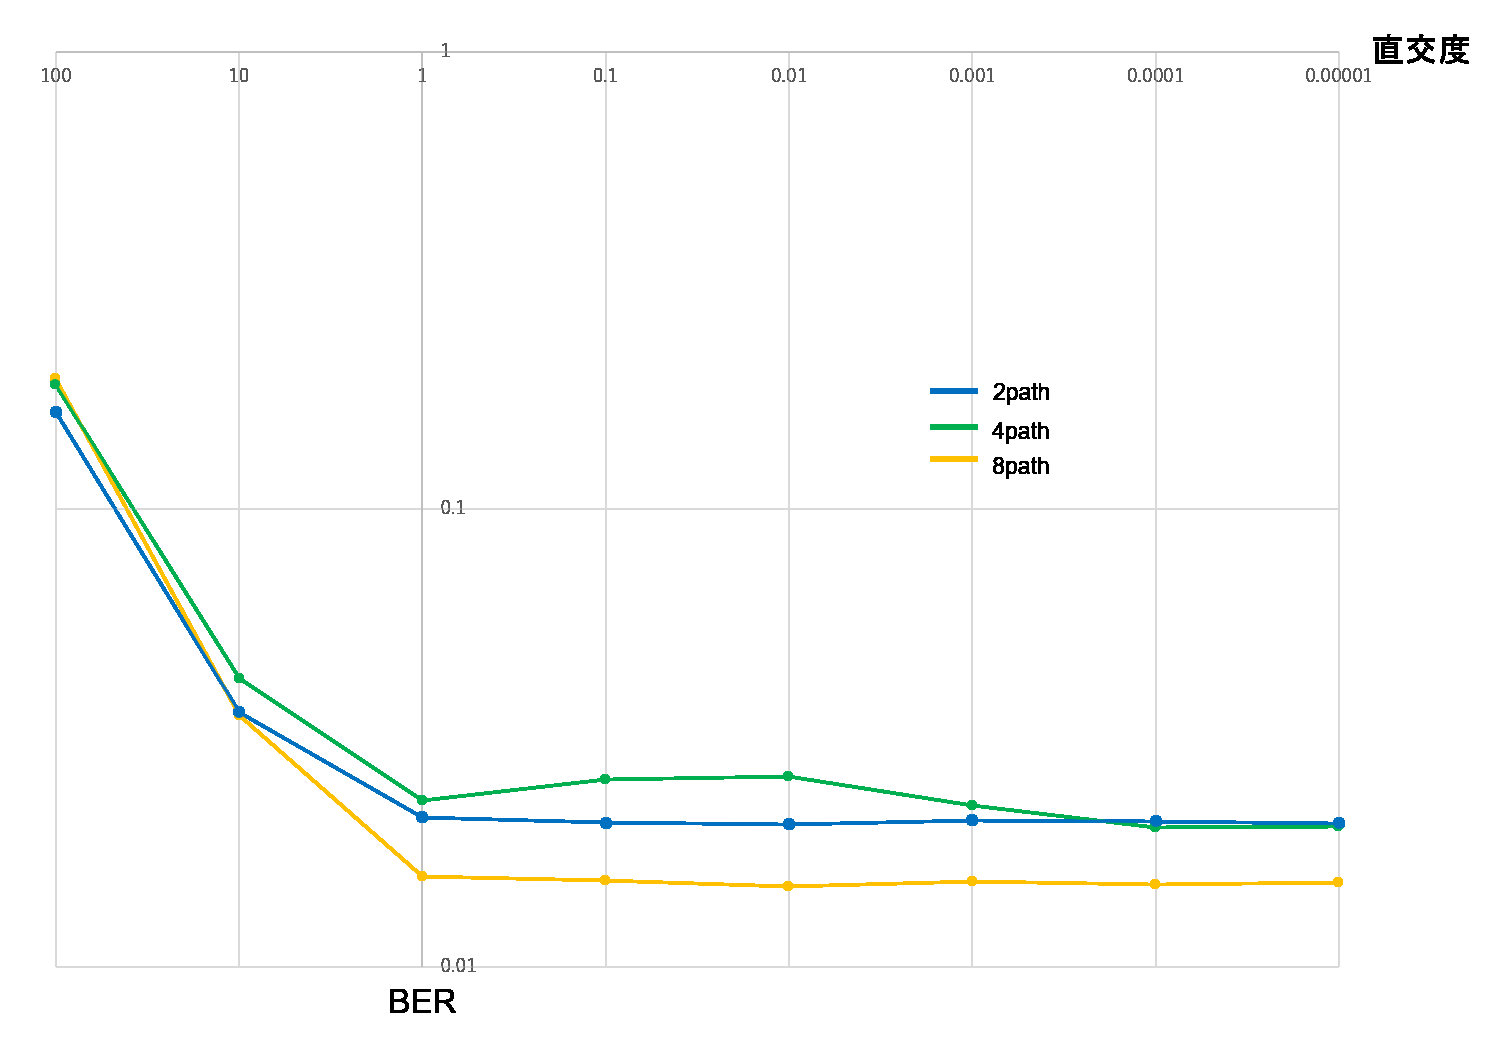
\includegraphics[width=0.95\linewidth]{chapter4/figure/CutoffSim2.eps}
    \caption{直交度とBERの関(マルチパス数変化時)}
    \label{figCutoffSim2}
\end{figure}

図 {figCutoffSim2}からわかるように,各マルチパス数について,BERが改善しなくなる点が
全ての条件でほぼ同じラインになっている.
つまり,収束基準がマルチパス数に依存しないことがわかる.
以上の検証結果から,収束基準は(4.21)式を用いることができると考えられる.

さて,ここまでで得た結果から足切りアルゴリズムのシミュレーション諸元を表 \ref{tabCutoff3}に
示す.

\begin{table}[ht]
    \begin{tabular}{|c|c|} \hline
        1ブロック当たりのシンボル数 & 32 \\ \hline
        マルチパス数 & 4 \\ \hline
        変調方式 & QPSK \\ \hline
        チャネルモデル & 準静的レイリーフェージング \\ \hline
        PPL時の雑音考慮 & 無し \\ \hline
        収束基準 & $exp(-0.23E_bN_0)$ \\ \hline
        BER基準 & 0.01 \\ \hline
    \end{tabular}
    \centering
    \caption{足切りアルゴリズムシミュレーション諸元}
    \label{tabCutoff3}
\end{table}

伝搬路は準静的レイリーフェージングモデルを考える.
また,収束基準とBER基準は本節でシミュレーションで求めた値を用いるものとする.

\subsubsection{シミュレーション結果}
ここでは(4.3.1)節の検証結果を基に設定した,固有ベクトルの収束基準と通信品質基準を用いて足切りアルゴリズムの
有効性について検証を行う.シミュレーション諸元は表 \ref{tabCutoff3}に示した通りである.

まず,図 \ref{figCutoffSim3}に$E_bN_0$と無線機間反復回数の関係を示す.

\begin{figure}[ht]
    \centering
    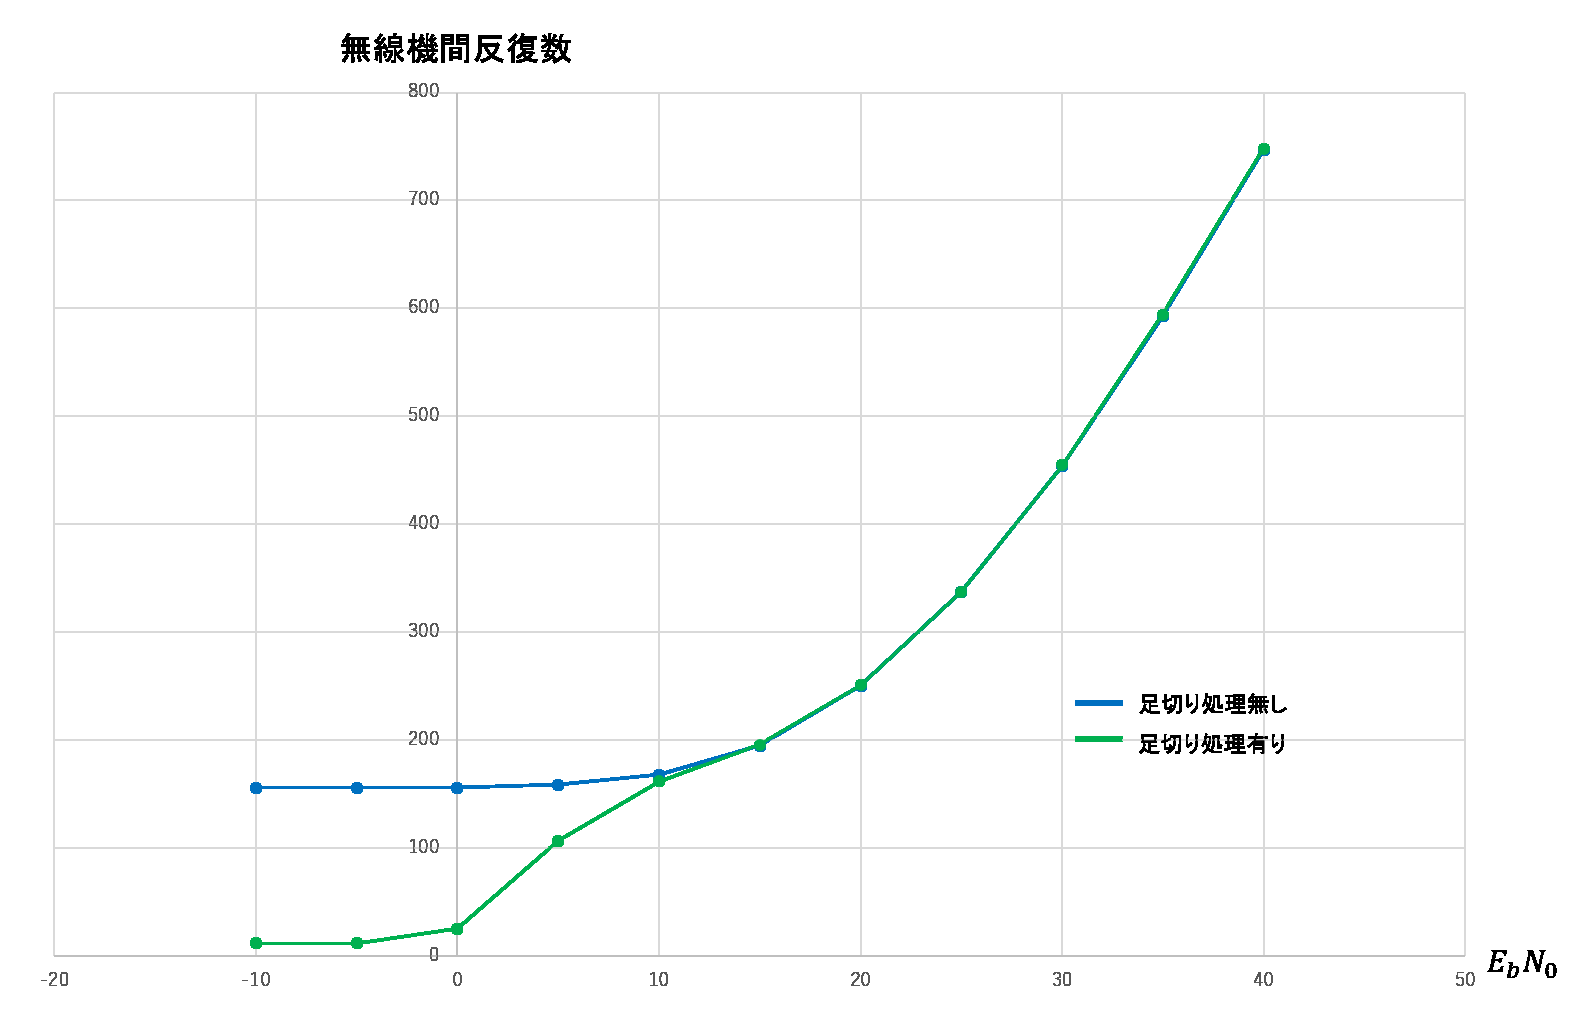
\includegraphics[width=0.95\linewidth]{chapter4/figure/CutoffSim3.eps}
    \caption{足切りアルゴリズム($E_bN_0$対無線機間反復数)}
    \label{figCutoffSim3}
\end{figure}

青のグラフが足切り処理有り,緑のグラフが足切り処理無しとなっている.
足切り処理無しの場合については,表 \ref{tabCutoff3}と同じ諸元でシミュレーションを行うが,
BER基準による足切り処理を行わないことと,全固有ベクトルが収束基準を満たすまで無線機間反復処理を
終了しないものとする.
グラフからわかるように,$E_bN_0$が小さい領域において反復回数を大きく削減できていることがわかる.
$E_bN_0$が大きい領域については,すべての固有ベクトルを使用しても
BERが通信品質基準より下回らないので,足切りが行われず,足切り処理を適用しない場合と同じ反復数が必要となる.

足切りアルゴリズムによって無線機間反復数が削減されることは示したが,使用可能なチャネル数,つまり,
設定した通信品質を満足するチャネル数が足切り処理を適用しない場合と適用した場合とで一致することを示す必要がある.
図 \ref{figCutoffSim4}に$E_bN_0$と使用可能チャネル数の関係を示す.なお,図 \ref{figCutoffSim4}は
図 \ref{figCutoffSim3}取得時のものであり,諸元も表 \ref{tabCutoff3}に示したものと同一である..

\begin{figure}[ht]
    \centering
    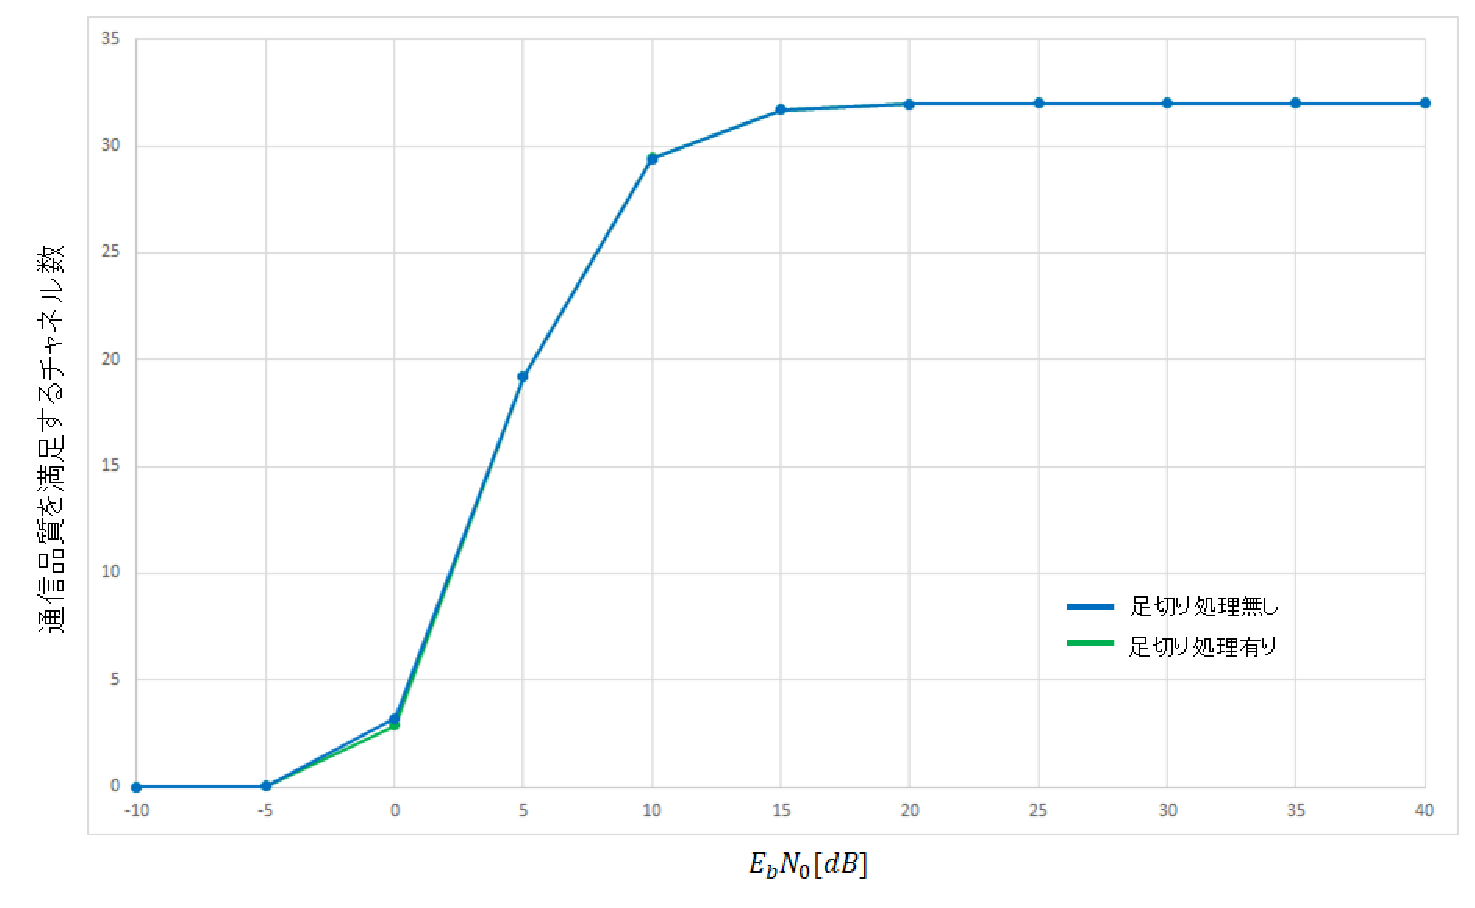
\includegraphics[width=0.95\linewidth]{chapter4/figure/CutoffSim4.eps}
    \caption{足切りアルゴリズム($E_bN_0$対使用可能チャネル数)}
    \label{figCutoffSim4}
\end{figure}

青のグラフが足切り処理無し,緑のグラフが足切り処理有りとなっている.
$E_bN_0$が小さい領域では,使用可能チャネル数が少なく,$E_bN_0$が大きくなるにつれて
使用可能チャネル数が多くなっていくのがわかる.これは,$E_bN_0$が小さいほど
誤り率が高くなってしまうので,実質的な通信品質基準を満足するチャネルが利得の大きい,
つまり固有値の大きいチャネルを使用した場合に限られるからである.
また,足切り処理有りと無しの場合を比較したとき,使用チャネル数は変わらないという結果になった.
つまり,図 \ref{figCutoffSim3}と図 \ref{figCutoffSim4}の結果から,足切りアルゴリズムを適用することで
使用可能チャネル数を減らすことなく,$E_bN_0$が小さい領域において無線機間反復数を削減できること
が確認できた.

\subsection{送信電力制御を用いたBER理論値最小化}
ここでは,利得の小さいチャネルの誤り率が高くなってしまう問題に対して,送信電力制御の
適用によるBER最小化について検証を行う.

\subsubsection{シミュレーション諸元}
理論的な内容については(4.2.2)節で説明したので,ここではシミュレーションの諸元を示すのみとする.
表 \ref{tabPcon1}に諸元を示す.

\begin{table}[ht]
    \begin{tabular}{|c|c|} \hline
        1ブロック当たりのシンボル数 & 32 \\ \hline
        マルチパス数 & 4 \\ \hline
        変調方式 & QPSK \\ \hline
        チャネルモデル & 準静的レイリーフェージング \\ \hline
        最小送信電力 & 0.01 \\ \hline
    \end{tabular}
    \centering
    \caption{送信電力分配シミュレーション諸元}
    \label{tabPcon1}
\end{table}

また,固有値・固有ベクトルについてはPPLではなく固有値分解によって獲得したものを使用する.
チャネル推定は誤差の全くない完全な精度で行われるとして,
各固有ベクトルは互いに完全に直交しているものとする.これは,PPLによる収束誤差による
影響を考慮せず,純粋に送信電力分配の効用を評価するためである.
また,送信電力分配時の最小送信電力の設定は,0.01としている.これは,1チャネル当たりの平均送信電力を1
としたとき,つまり全チャネル合計で32の送信電力として設定したものである.

\subsubsection{シミュレーション結果}
図 \ref{figPconSim1}にシミュレーション結果を示す.

\begin{figure}[ht]
    \centering
    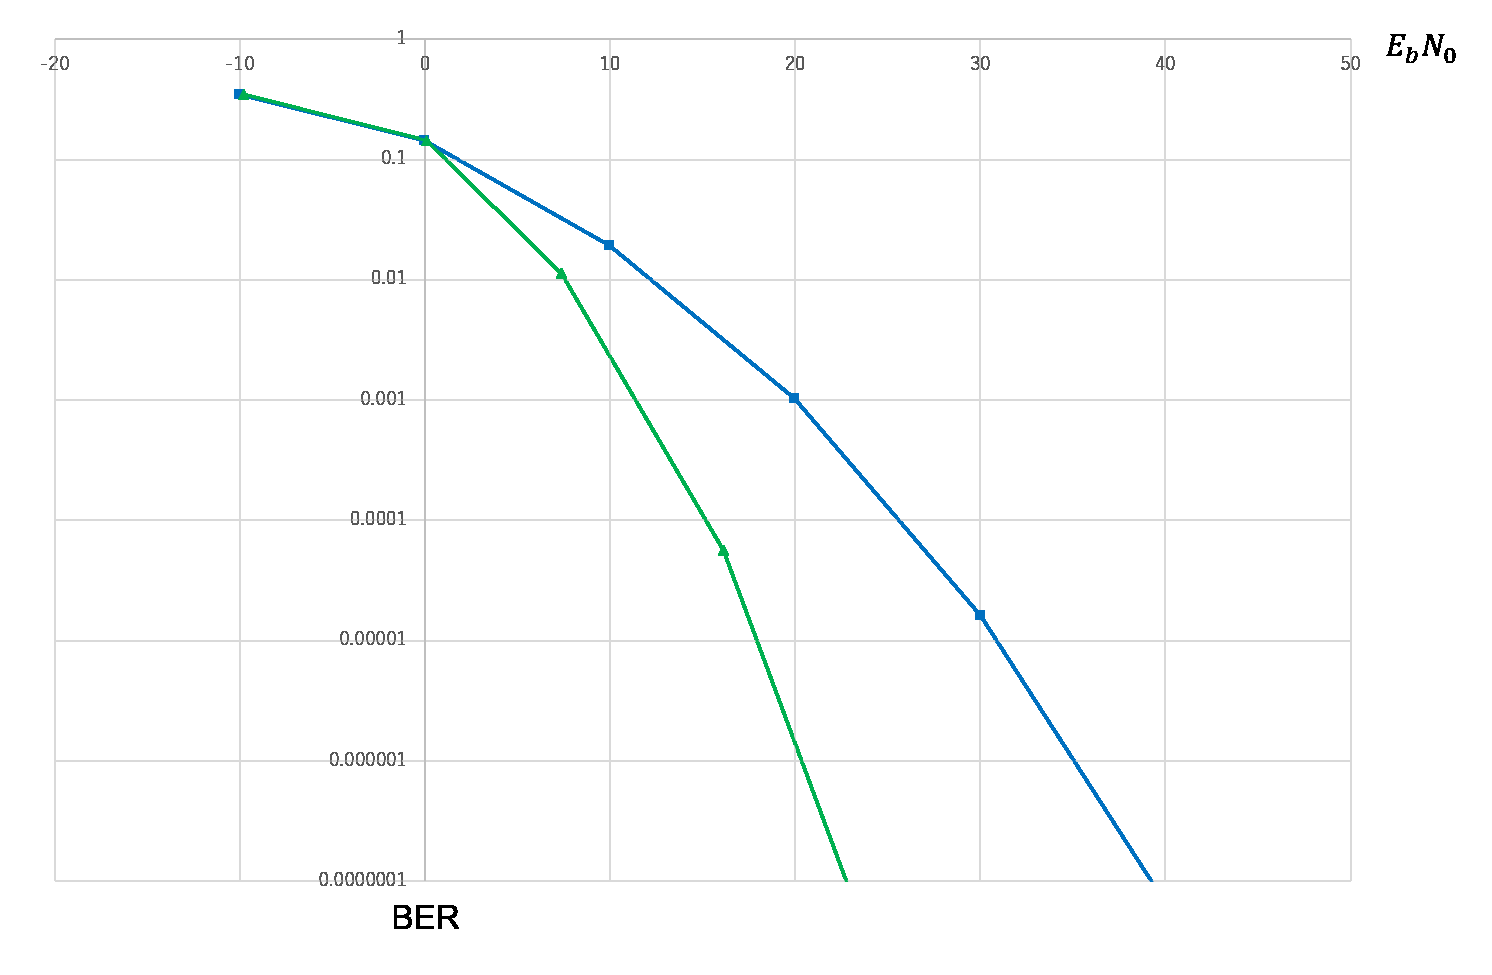
\includegraphics[width=0.95\linewidth]{chapter4/figure/PconSim1.eps}
    \caption{送信電力分配}
    \label{figPconSim1}
\end{figure}

青のグラフが送信電力分配無し,緑のグラフが送信電力分配適用ありとなっている.
グラフからわかる通り,送信電力分配適時の方がBERを小さく抑えることができている.
$E_bN_0$が小さい領域では,送信電力分配を適用する場合としない場合で同じ結果となっているが,
これは,雑音による影響が強すぎるためだと考えられる.

\subsection{送信電力制御適用時の使用チャネル足切りアルゴリズム}
ここでは,これまで検証した足切りアルゴリズムと送信電力制御を同時適用した場合について
シミュレーションを用いて検証を行う.
足切りアルゴリズムに送信電力制御を組み込む目的としては,足切りによって無線機間反復回数を
削減しつつ,使用可能チャネルを最大化することにある.

\subsubsection{シミュレーション諸元}
シミュレーション諸元を表 \ref{tabComb1}に示す.
伝搬路は準静的レイリーフェージングモデルとする.
また,送信電力分配時の最小送信電力の設定は,0.01としている.これは,1チャネル当たりの平均送信電力を1
としたとき,つまり全チャネル合計で32の送信電力として設定したものである.
収束基準とBER基準は4.3.1.1節で検証した結果を使用する.

\begin{table}[ht]
    \begin{tabular}{|c|c|} \hline
        1ブロック当たりのシンボル数 & 32 \\ \hline
        マルチパス数 & 4 \\ \hline
        変調方式 & QPSK \\ \hline
        チャネルモデル & 準静的レイリーフェージング \\ \hline
        PPL時の雑音考慮 & 無し \\ \hline
        収束基準 & $exp(-0.23E_bN_0)$ \\ \hline
        BER基準 & 0.01 \\ \hline
        送信電力分配最適化時最小送信電力 & 0.01 \\ \hline
    \end{tabular}
    \centering
    \caption{送信電力分配適用時足切りシミュレーション諸元}
    \label{tabComb1}
\end{table}

\subsubsection{シミュレーション結果}
ここでは,表 \ref{tabComb1}の諸元に基づいたシミュレーションを行った結果を示す.
図 \ref{figCombSim1}に$E_bN_0$対無線機間反復数の関係,図 \ref{figCombSim2}
に$E_bN_0$対使用可能チャネル数の関係を示す.
ここでの使用可能チャネル数とはBER基準を満足するチャネル数を表している.

\begin{figure}[ht]
    \centering
    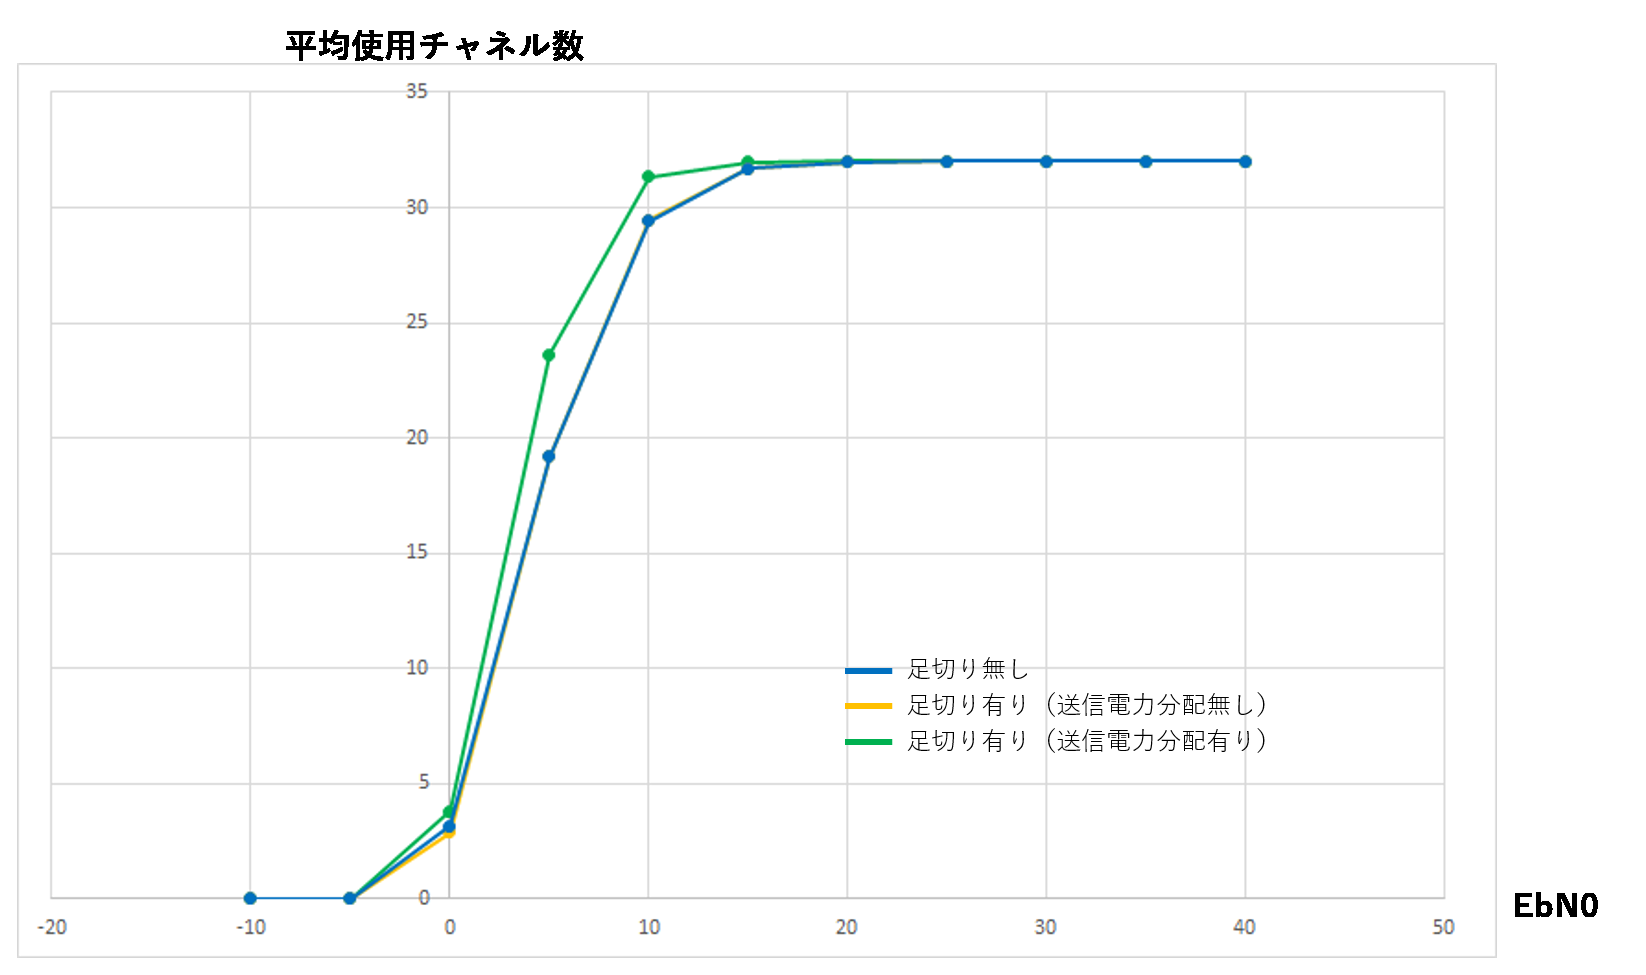
\includegraphics[width=0.95\linewidth]{chapter4/figure/CombSim1.eps}
    \caption{送信電力分配適用時足切りアルゴリズム($E_bN_0$対無線機間反復数)}
    \label{figCombSim1}
\end{figure}

\begin{figure}[ht]
    \centering
    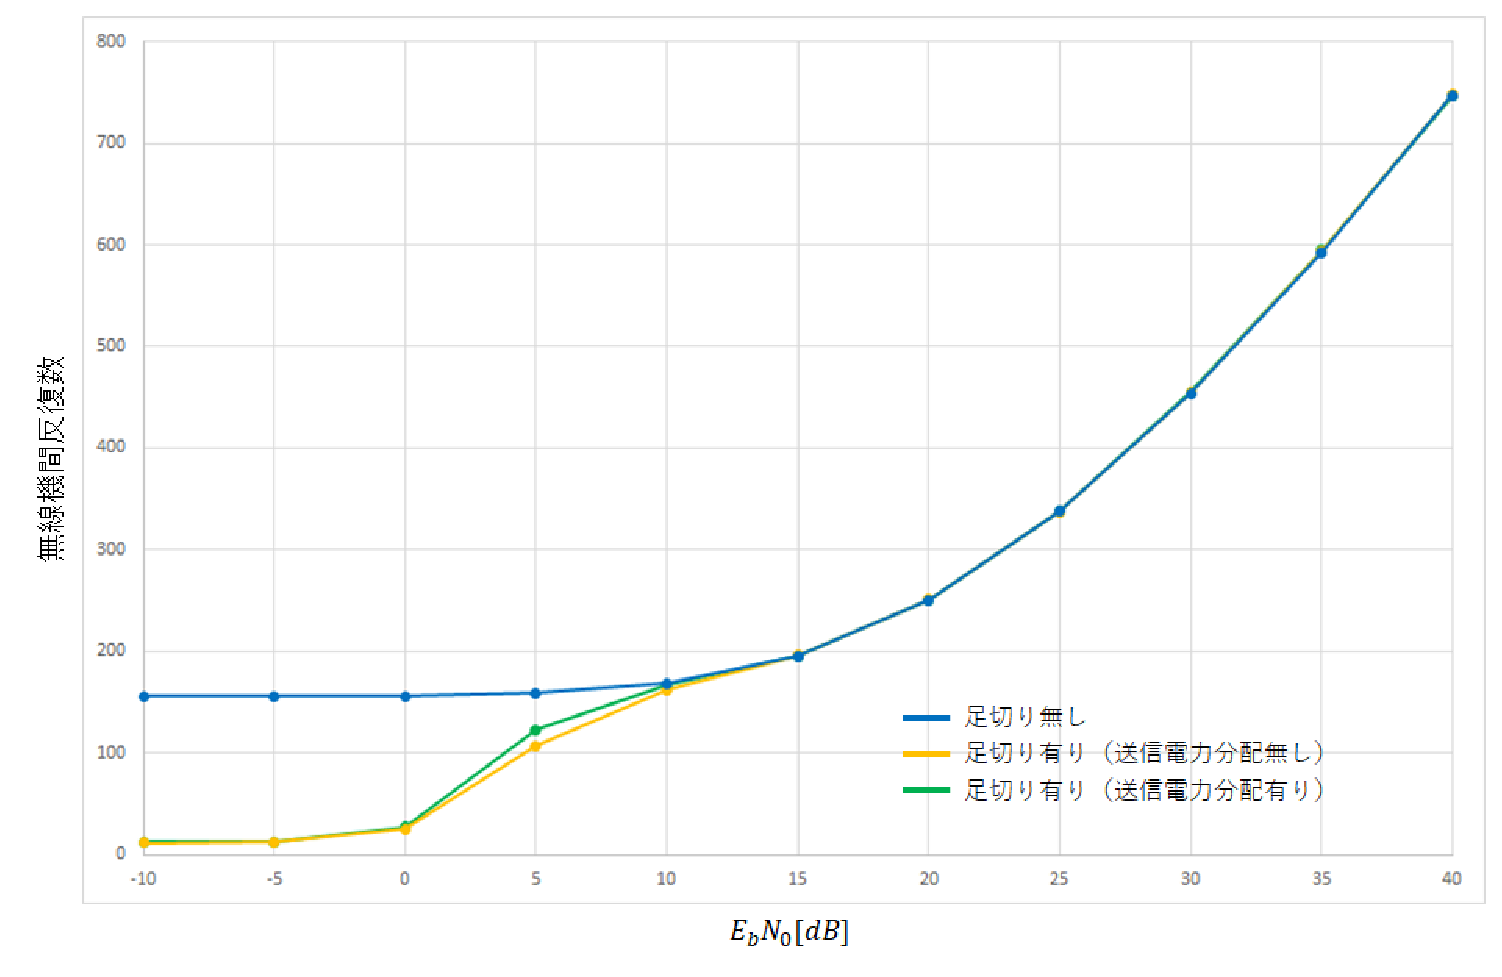
\includegraphics[width=0.95\linewidth]{chapter4/figure/CombSim2.eps}
    \caption{送信電力分配適用時足切りアルゴリズム($E_bN_0$対使用可能チャネル数)}
    \label{figCombSim2}
\end{figure}

まず,図 \ref{figCombSim1}から見る.青のグラフが足切りも送信電力分配も適用しない時,
黄のグラフが足切りは適用するが送信電力分配は適用しない場合,そして緑のグラフが
足切りと送信電力分配を同時適用した場合となっている.
図 \ref{figCombSim1}からわかるように,$E_bN_0$が$-5[dB]~20[dB]$の領域において,
送信電力分配を適用した場合で使用可能チャネル数が増えていることがわかる.
これは,送信電力分配によってBERが最小化されたために,BER基準を満足するチャネルが
増えたためだと考えられる.

また,図 \ref{figCombSim2}には,送信電力分配を同時適用した場合の無線機間反復数が
示されている.$E_bN_0=5[dB]$の点で,若干送信電力分配を適用しない場合に比べて
反復回数が増えているが,図 \ref{figCombSim1}の使用可能チャネル数の増加度合いに
比べると,十分小さい増え幅だと言える.
つまり,送信電力分配を足切りアルゴリズムに適用することによって,
使用可能チャネル数を最大化しつつ,無線機間反復数を抑えることができた.

ここまでの足切りアルゴリズムでは,$E_bN_0$が小さい領域で無線機間反復数を削減できた.
しかし,$E_bN_0$が大きい領域においては,$E_bN_0$が大きくなるにつれて無線機間反復数も
増大している.これは,図 \ref{figCutoffSim3}に示したように,
$E_bN_0$が大きくなるにつれて,固有ベクトルの直交誤差がBERに影響しないように,
収束基準が厳しくなっていくためである.
しかし,QPSKにおいて0.01のBER基準を満足することに焦点を当てた場合,ある程度の
収束誤差があっても,BER基準さえ満足すれば誤り訂正によって誤り率を0にすることができる.
ここでは,最大無線機間反復数を設定することで,具体的に何回程度の反復処理を行えば,
その時点で獲得したことが固有ベクトルがBER基準を満足するのかシミュレーションを用いて
求めてみる.
シミュレーション諸元は表 \ref{tabComb1}と同じとするが,最大反復回数を超える場合は,
その時点で収束基準に関係なく反復処理を終了する.
また,最大反復回数を超えて反復処理が打ち切りになった場合は,送信電力分配は行わない
こととする.これは,途中で反復処理が打ち切られた場合,固有値が正しく求められていない
チャネルが存在するので,定数として固有値を使用する最適化問題の解が不正になるためである.
図 \ref{figComb3}にシミュレーション結果を示す.

\begin{figure}[ht]
    \centering
    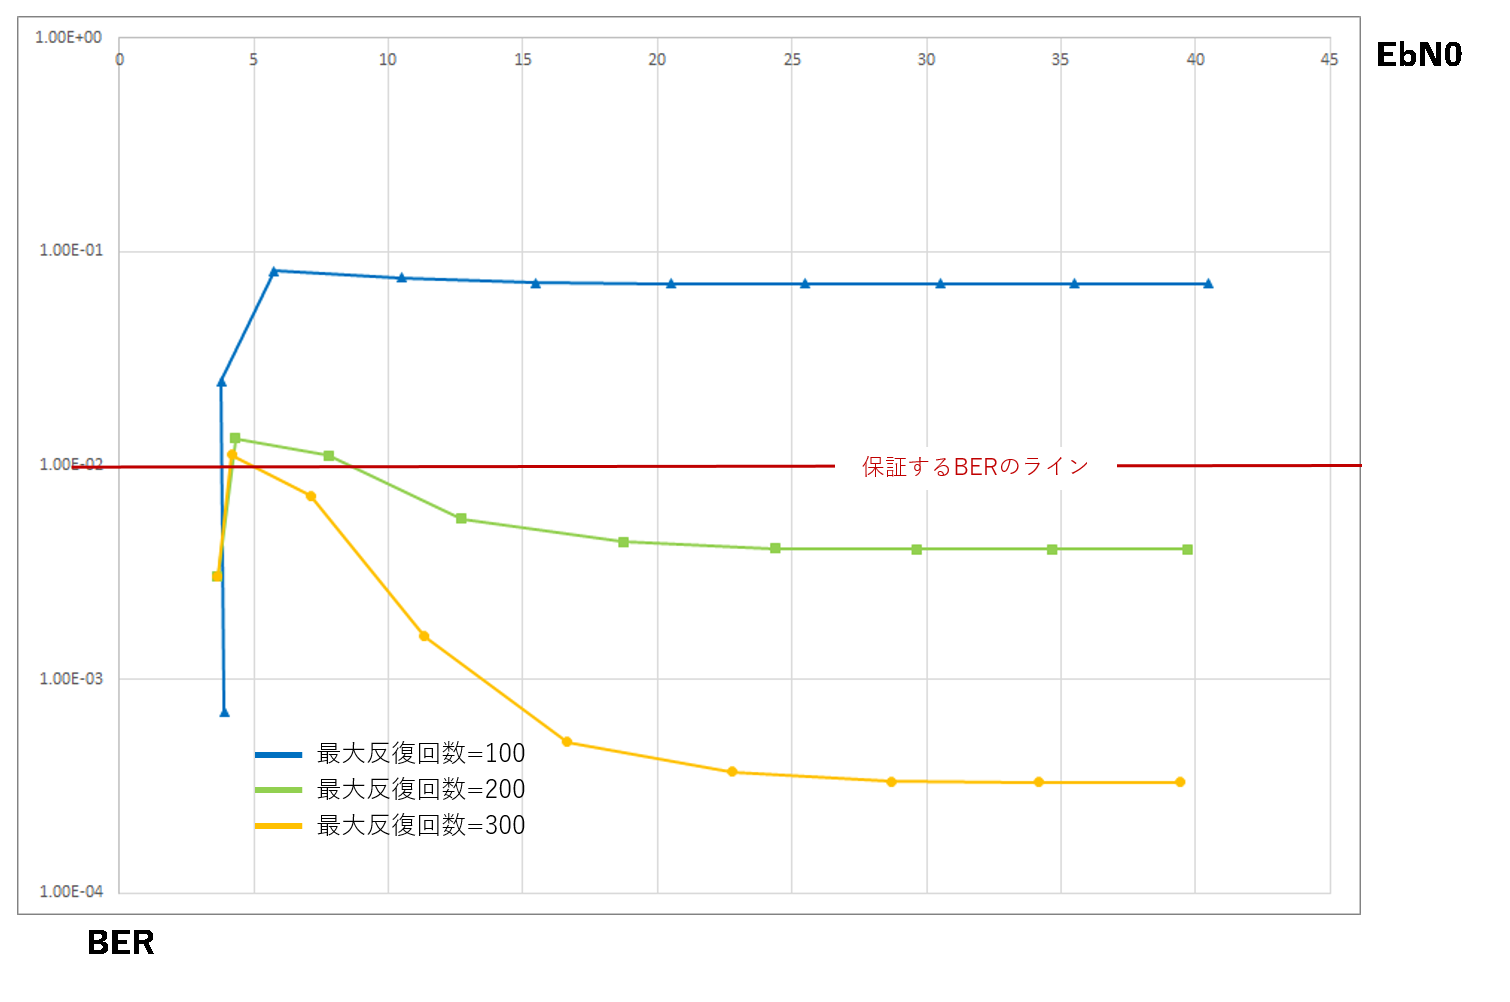
\includegraphics[width=0.95\linewidth]{chapter4/figure/CombSim3.eps}
    \caption{送信電力分配適用時足切りアルゴリズム($E_bN_0$対BER)}
    \label{figCombSim3}
\end{figure}

それぞれ,青のグラフが100回,緑のグラフが200回,黄のグラフが300回の最大反復回数となっている.
この内,200回と300回についてはBER基準を満たしているが,100回では固有ベクトルの収束誤差が
大きくBER基準を満たすことができなかった.
以上の結果から,200回程度を最大反復回数に設定することで,BER基準を満たしつつ$E_bN_0$が
大きい領域でも無線機間反復数を低減できると考えられる.
図 \ref{figCombSim4}に最大反復回数を200回に設定した場合のシミュレーション結果を示す.
なお,シミュレーション諸元は表 \ref{tabComb1}と同一の条件を使用した.

\begin{figure}[ht]
    \centering
    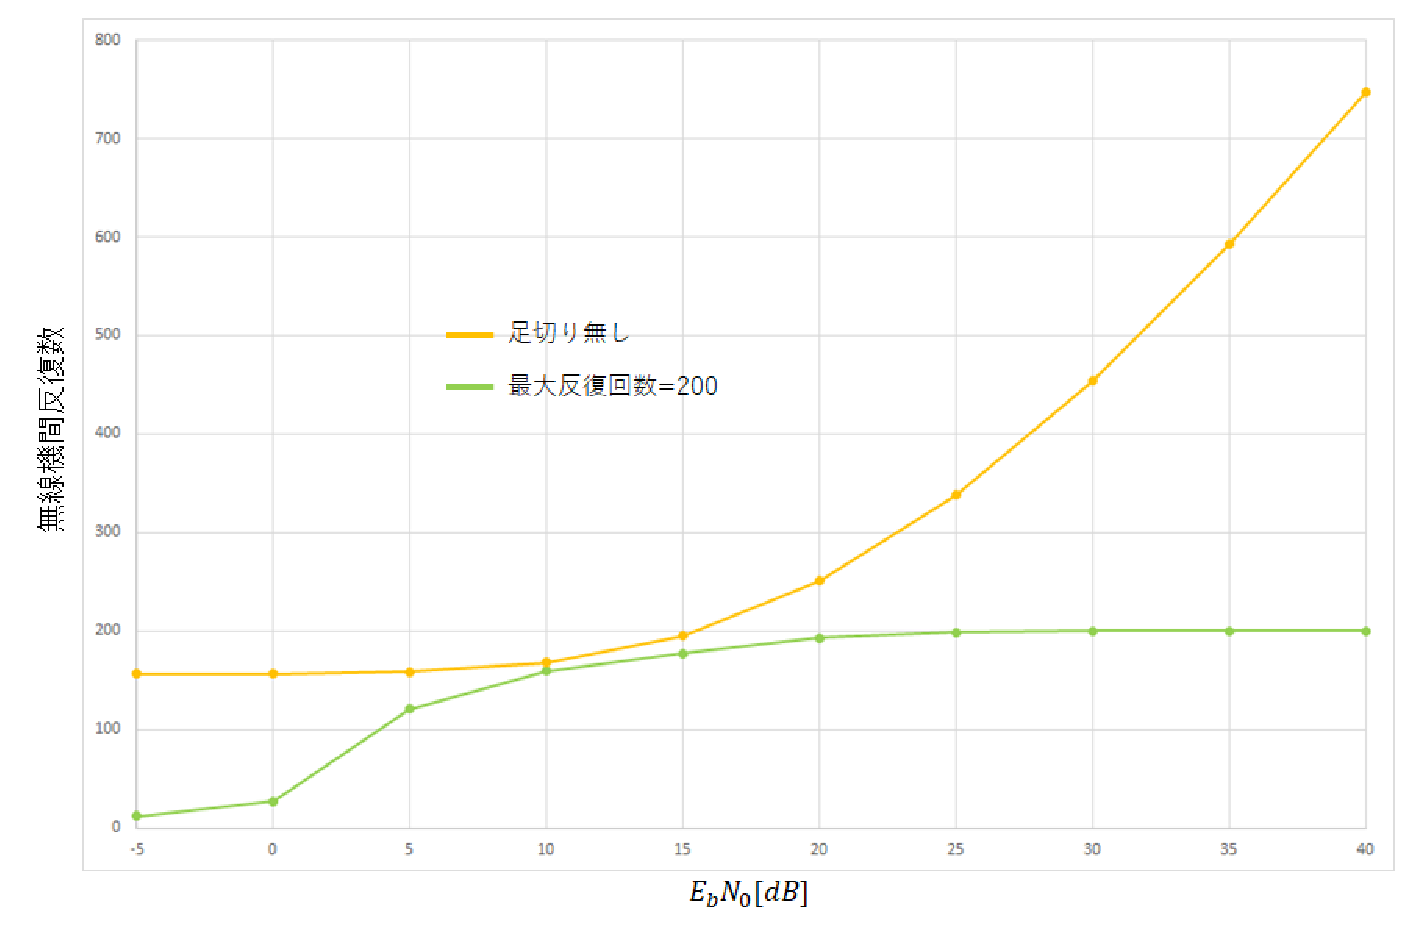
\includegraphics[width=0.95\linewidth]{chapter4/figure/CombSim4.eps}
    \caption{送信電力分配適用時足切りアルゴリズム(最大反復回数設定)}
    \label{figCombSim4}
\end{figure}

黄のグラフが足切りアルゴリズム適用無し,緑のグラフが最大反復回数を200回に設定した際の
送信電力適用時足切りアルゴリズムになっている.

図 \ref{figCombSim4}から,$E_bN_0$が大きい領域について無線機間反復数が200回に
抑えられていることがわかる.今回は変調方式にQPSKを使用したため,200回程度の最大反復回数で
十分BER基準を満たすことができたが,16QAMのように変調多値数が大きくなってくると,
必要な最大反復回数も増加することが予想される.

本章で行った3つの検証を通して,送信電力制御を足切りアルゴリズムに組み込むことで,
使用可能チャネル数を最大化しつつ,無線機間反復数は当該アルゴリズムを適用しない場合に
比べて大幅に削減できることが示された.PPLは,チャネル推定を行って固有値分解によって
固有ベクトルを求める方式と比べて,膨大な演算量を比較的簡単な非線形処理と無線機間反復処理に
置き換えられる点にメリットがある.具体的な状況としては,高速な無線通信には向かないが,
中程度のデータ量を扱う回線において,無線機にハード的な制約によって高い演算能力を
持たせることができない場合について有効だと言える.